\documentclass[tikz,border=2pt]{standalone}
\usepackage{amsmath,amssymb}
\usepackage{tikz}

\begin{document}
% Kruskal: scan the edges in increasing length and keep each one that does not close a cycle
% with the edges already kept.
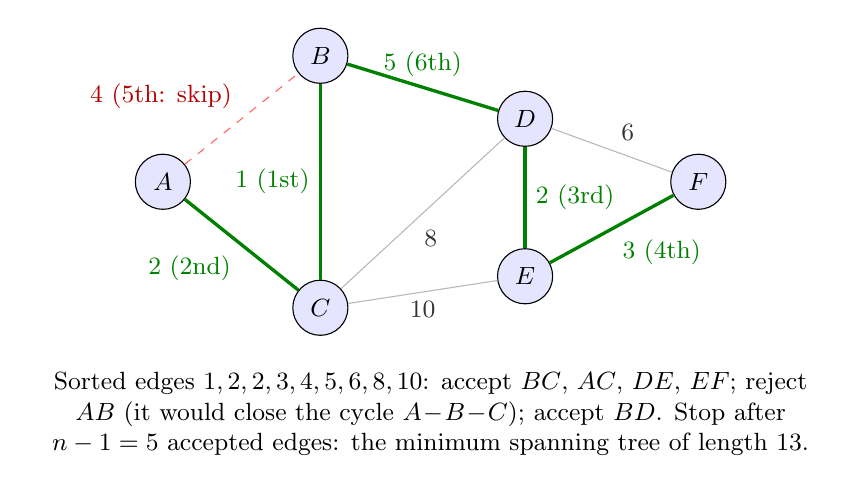
\begin{tikzpicture}[every node/.style={font=\small}, v/.style={draw, circle, fill=blue!10, minimum size=7mm, inner sep=0pt}]
	\node[v] (A) at (0,0) {$A$};
	\node[v] (B) at (2,1.6) {$B$};
	\node[v] (C) at (2,-1.6) {$C$};
	\node[v] (D) at (4.6,0.8) {$D$};
	\node[v] (E) at (4.6,-1.2) {$E$};
	\node[v] (F) at (6.8,0) {$F$};
	\draw[red!60, dashed] (A) -- (B) node[midway, above left, text=red!70!black] {$4$ (5th: skip)};
	\draw[gray!55] (C) -- (D) node[pos=0.45, below right, text=gray!40!black] {$8$};
	\draw[gray!55] (C) -- (E) node[midway, below, text=gray!40!black] {$10$};
	\draw[gray!55] (D) -- (F) node[midway, above right, text=gray!40!black] {$6$};
	\draw[green!50!black, very thick] (B) -- (C) node[midway, left] {$1$ (1st)};
	\draw[green!50!black, very thick] (A) -- (C) node[midway, below left] {$2$ (2nd)};
	\draw[green!50!black, very thick] (D) -- (E) node[midway, right] {$2$ (3rd)};
	\draw[green!50!black, very thick] (E) -- (F) node[midway, below right] {$3$ (4th)};
	\draw[green!50!black, very thick] (B) -- (D) node[midway, above] {$5$ (6th)};
	\node[anchor=north, align=flush center, text width=10cm] at (3.4,-2.3) {Sorted edges $1,2,2,3,4,5,6,8,10$: accept $BC$, $AC$, $DE$, $EF$; reject $AB$ (it would close the cycle $A\!-\!B\!-\!C$); accept $BD$. Stop after $n-1=5$ accepted edges: the minimum spanning tree of length $13$.};
\end{tikzpicture}
\end{document}
